\documentclass[a4paper]{scrartcl}
\usepackage[utf8]{inputenc}
\usepackage{xcolor}
\usepackage{graphicx}
\graphicspath{{./figures/}}

\title{Assignment 1}
% \textcolor{gray}{Critique and re-design of an existing graphic}
\author{Alina Mokrova\\
				01325014
				\and
				Levente	Slajchó\\
				01634250
				\and
				Maximilian Walterskirchen\\
				id
				\and
				Leminh Nguyen\\
				11945068}
\date{\today}

\begin{document}

\maketitle

\section{Analysis and criticism}


\subsection{Analysis of the infographic}

The infographic \textit{Nutritional Values} by Dan Mariglio in
Figure~\ref{assignmentGraphic} pictures the nutritional comparison between
processed and natural/wholesome food. The author visualizes three different
infographics for the different food categories; the first graph compares the
cost per calorie, another one contrasts the calories per \textit{100g} and the
last shows how much sugar is contained in \textit{100g}. The author gives the
example that wholesome food is more expensive since the ratio of value to
calorie for an apple is higher compared to a bag of potato chips. Mariglio based
his visualizations on the layout of common supermarkets and suggests the reader
sticking to the periphery of the supermarket to find the natural food.
Processed food containing the most calories by weight is located at the centre
of the grocery store.

\subsection{Criticism of the visual design}

In this section, the three infographics will be criticised according to the
visual design principles from the lecture notes. These design principles were
defined by Edward Tufte\cite{Tufte2001}.

\subsubsection{Perception and cognition}

\textcolor{gray}{
The author uses the data-driven, Bottom-up approach
The graphics are a conventional representation and used the controlled visualization paradigm (reason: data-driven)
Which requires the attentive perception of the reader/viewer
The attentive approach is slow to perceive and easy to forget information
Based on visual processing paradigm and requires the following from the viewer:
Parallel processing to extract low-level properties of the visual scene
Pattern perception
Deficiency for viewers with colour blindness, see produce aisle/section which is represented in red and green
The graphic in 3 dimensions which makes itway more complex than it is
Principles of Graphical Integrity (Tufte principles of design)
The food graphical components obscure the actual information and data -> hard to perceive actual infographic
Preattentive processing:
No immediate understanding
No preattentive attributes, except food labels but many, are obscured by other components
Hard for immediate perception
}

% The differences between the three tables are difficult to compare due to too much information and bright colour
% Data-Users-Tasks triangle:
% Expressiveness – Are the visual elements expressive enough?  >> even too much
% Effectiveness – Is the information displayed effectively? >> not at all
% Appropriateness – Is the visualization appropriate? >> yes, its perfect for the subject

\subsubsection{Design priniciples by Edward Tufte}

% Principles of Graphical Excellence:

% Complex ideas communicated with clarity, precision and efficiency.
% The viewer grasps the ideas of the visualization quick with the least amount of ink in the smallest space

% Principles of Graphical Integrity:

% Lie Factor
% Clear detailed and labelled
% show data variation, not design variation
% not exceed the number of dimensions of the data

% Principles of Data Graphics:

% Show me the numbers:
% ‘Above all show the data’
% Ink should present new information
% Elimination of non-data ink without loss of the data
% The elegance of visual design, defined by reached state where no elements cannot be removed and not the other way around of nothing to add
% Deemphasize non-data ink
% Push non-data ink into the background (supermarket blueprint)
% Display data in the foreground
% Nothing stands out since data-ink and non-data ink are given the same weight
% The viewers' eyes are drawn to contrast found in the 3d components which leads the reader from the actual data
% Different colours even though the same dataset leads the reader to think the difference it dataset
% Chartjunk 

% `A good graph is quiet and lets the data tell their story clearly and
% completely.`-Wainer, 1997
% Tufte Design Principles 
% 1. Above all else show the data 
% 2. Maximize the data-ink ratio 
% 3. Erase non-data-ink 
% 4. Erase redundant data-ink 
% 5. Maximize data density, within reason (Data density = number of entries/area of data graphic) 
% 6. Revise and edit

% Rules by Stephen Few about using colour in charts and graphs

% Use different colours only when they correspond to differences of meaning
% in the data 
% here for example for the vegetables multiple colours are used
% although that's not necessary

% To guarantee that most people who are colourblind can distinguish groups of data
% that are colour-coded, avoid using a combination of red and green in the same
% display.

% Use soft natural colours to display most information and bright and/or dark
% colours to highlight information that requires greater attention

\section{Assessment of redesign}

@Levente this is your section, I will add some notes for you here:

How we decided to re design the infographic:

\begin{itemize}
	\item deemphasize the non data-ink
	\item augment the data-ink
	\item declutter
	\item regroup the data
\end{itemize}

% link to appendix of new design

\bibliographystyle{ieeetr}
\bibliography{ivassignment}

\newpage
\clearpage
\section{Appendix}

\begin{figure}[h]
  \centering
	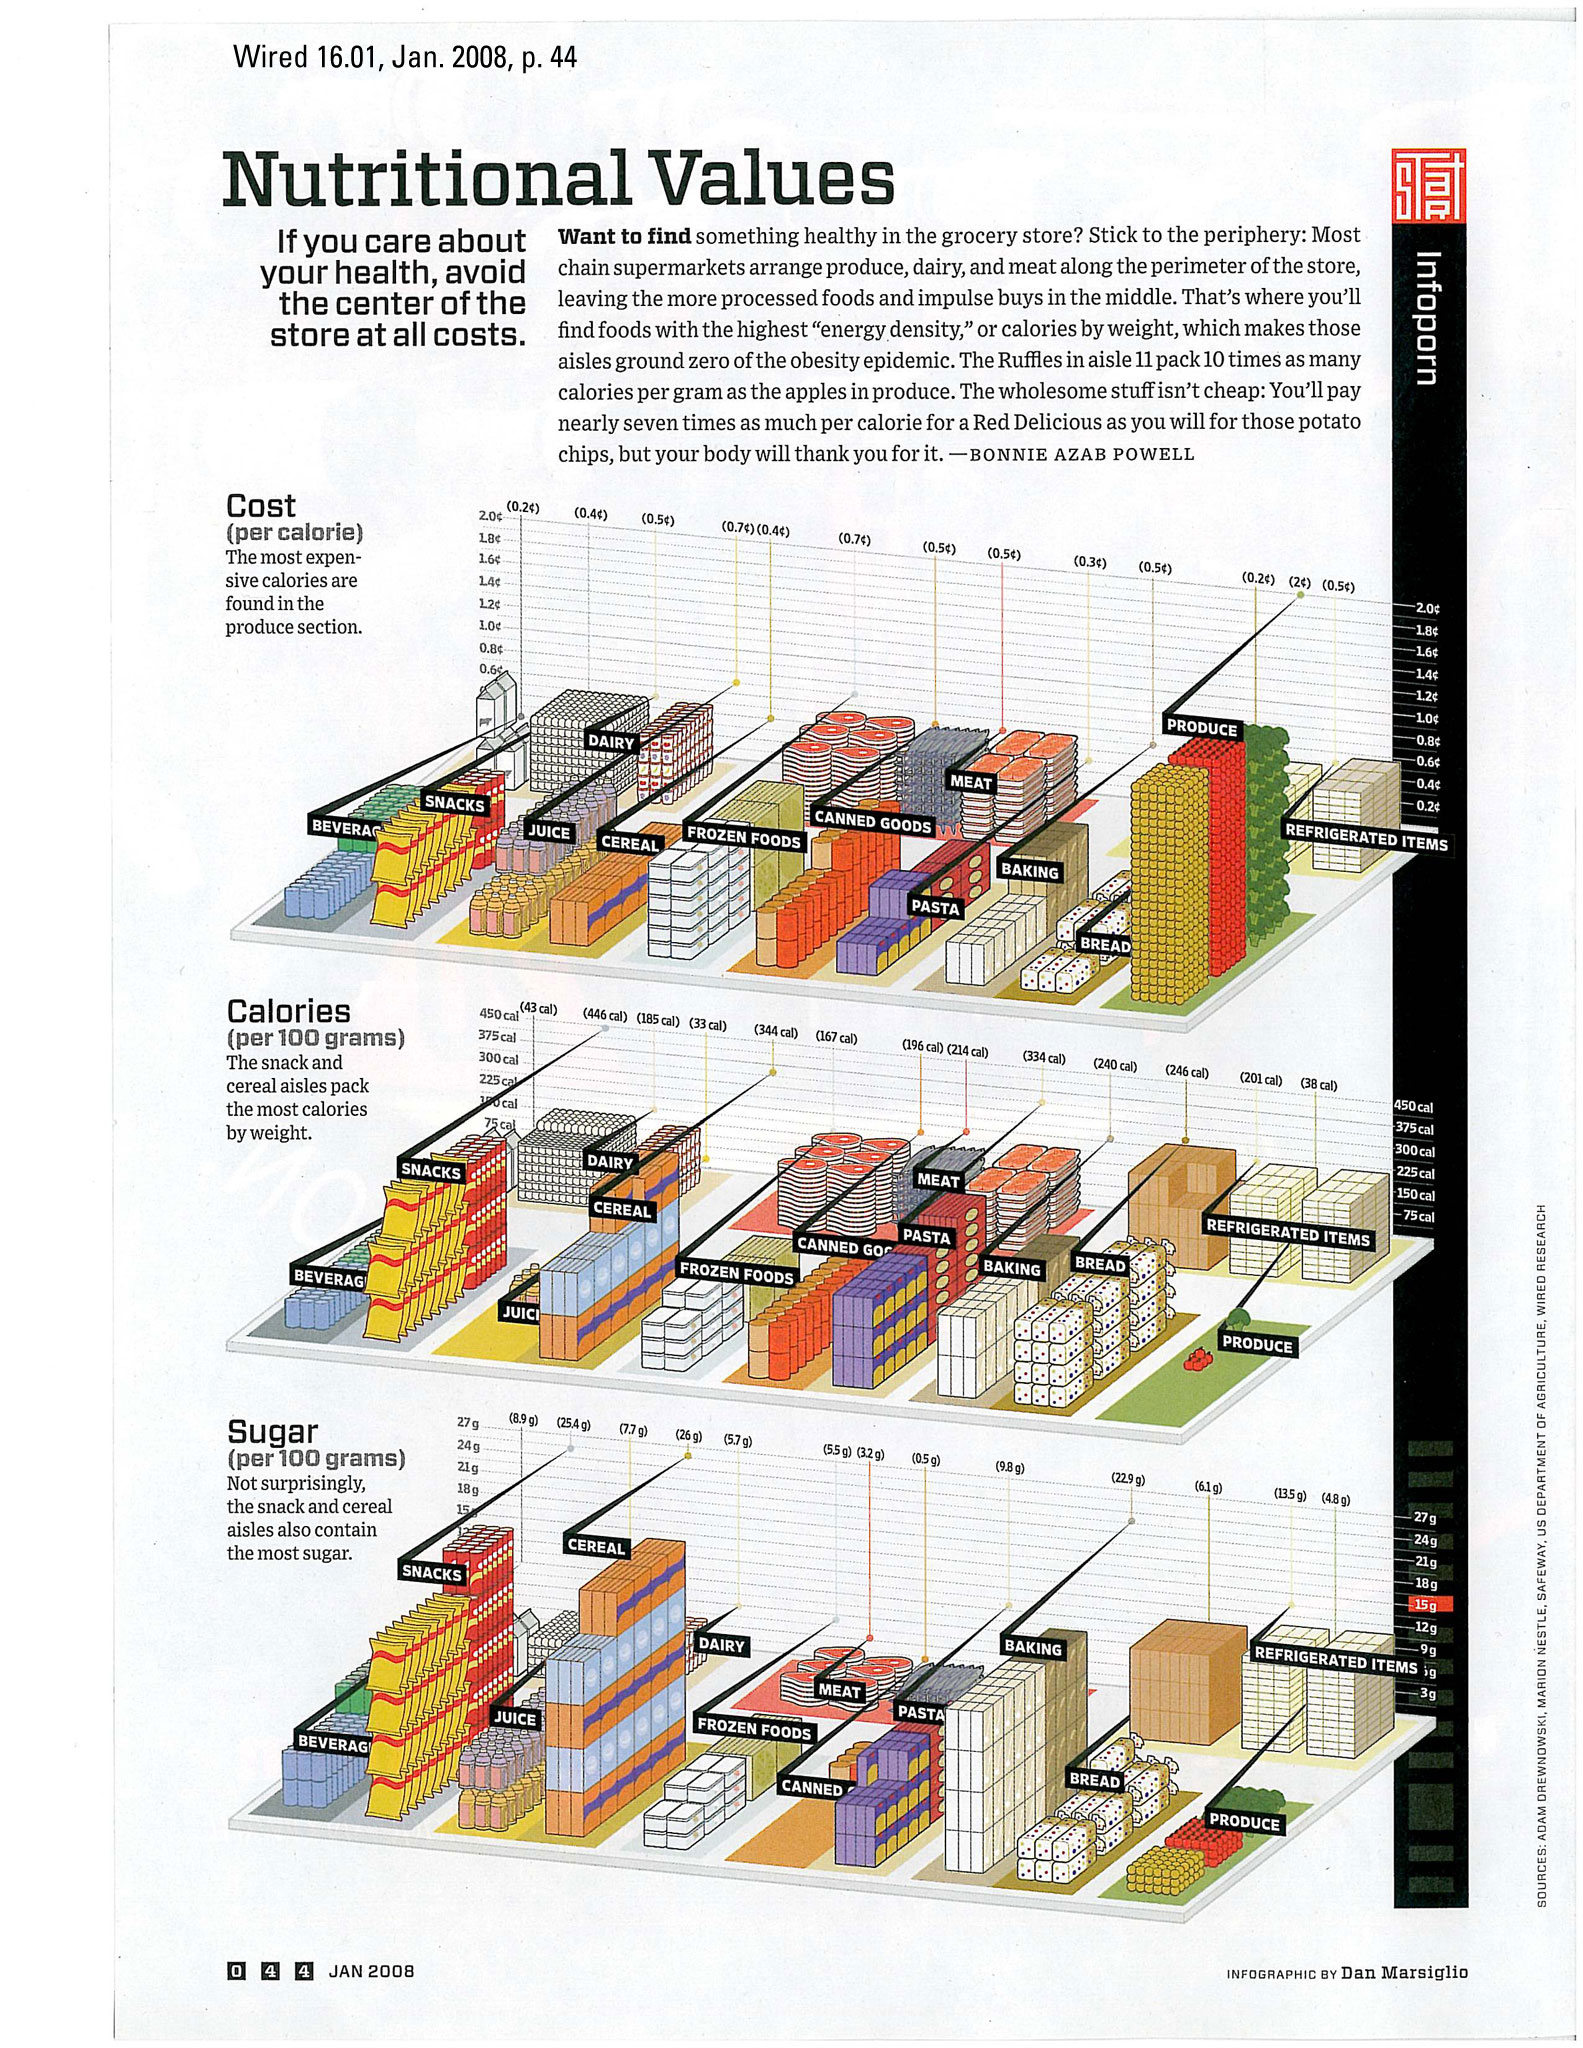
\includegraphics[scale=0.20]{assignmentGraphic.jpg}
  \caption{Given graphic to criticize.}
	\label{assignmentGraphic}
\end{figure}

\end{document}
